\documentclass[9pt]{extarticle}

\usepackage[a4paper,top=15mm,bottom=16mm,left=16mm,right=16mm]{geometry}
\usepackage[T1]{fontenc}
\usepackage{lmodern}
\usepackage{microtype}
\usepackage{graphicx}
\usepackage{booktabs}
\usepackage{tabularx}
\usepackage{longtable}
\usepackage{array}
\usepackage{enumitem}
\usepackage{xcolor}
\usepackage{titlesec}
\usepackage{fancyhdr}
\usepackage{hyperref}

\definecolor{ink}{HTML}{172B4D}
\definecolor{blue}{HTML}{276FBF}
\definecolor{softblue}{HTML}{EAF2FB}
\hypersetup{colorlinks=true,urlcolor=blue,linkcolor=blue,pdfauthor={Alexander Suvorov}}
\graphicspath{{imgs/}}
\urlstyle{same}
\setlength{\parindent}{0pt}
\setlength{\parskip}{3pt}
\setlength{\tabcolsep}{4pt}
\renewcommand{\arraystretch}{1.10}
\setlist[itemize]{leftmargin=*,nosep}
\titleformat{\section}{\Large\bfseries\color{ink}}{\thesection}{0.5em}{}
\titleformat{\subsection}{\large\bfseries\color{ink}}{\thesubsection}{0.45em}{}
\titlespacing*{\section}{0pt}{9pt}{3pt}
\titlespacing*{\subsection}{0pt}{6pt}{2pt}
\pagestyle{fancy}
\fancyhf{}
\fancyhead[L]{\scriptsize Alexander Suvorov}
\fancyhead[R]{\scriptsize Technical Appendix: Few-Shot SmolVLA}
\fancyfoot[C]{\scriptsize A-\thepage}
\renewcommand{\headrulewidth}{0.2pt}
\setlength{\headheight}{11pt}

\newcommand{\code}[1]{\texttt{\detokenize{#1}}}
\newcommand{\sha}[1]{\nolinkurl{#1}}
\newcommand{\artifact}[1]{\texttt{\small\detokenize{#1}}}
\newcommand{\yes}{\textcolor{blue}{\textbf{yes}}}

\begin{document}

\begin{center}
{\fontsize{22}{25}\selectfont\bfseries\color{ink} Technical Appendix}\\[2pt]
{\large One Shot Is All You Need. Or Is It?}\\[5pt]
{\normalsize\textbf{Alexander Suvorov} \quad HSE University}\\[5pt]
\href{https://github.com/alexsuw/smolvla-libero-fewshot}{GitHub repository}
\quad $\cdot$ \quad
\href{https://huggingface.co/collections/alexsuw/smolvla-libero-few-shot-6a8b009357482d2b4b9d3c2f}{Hugging Face collection}
\end{center}

\begin{center}
\colorbox{softblue}{\begin{minipage}{0.94\textwidth}
\small
This appendix records the exact protocols, counts, per-task/per-seed results,
training curves, compute measurements, and integrity checks behind the four-page
main report. It is not part of the four-page submission limit.
All target tables use environment success and show raw counts.
\end{minipage}}
\end{center}

\section{Frozen protocol and provenance}

\subsection{Immutable sources}

\begin{center}
\small
\begin{tabularx}{\textwidth}{@{}lX@{}}
\toprule
Item & Frozen value\\
\midrule
Base model & \code{lerobot/smolvla_base}, revision \sha{c83c3163b8ca9b7e67c509fffd9121e66cb96205}\\
Dataset & \code{nvidia/LIBERO_LeRobot_v3}, revision \sha{e5907374380b8f96511957e6ba5582be52a1e179}\\
Seen suite & Full available \code{libero_90}: 3,921 episodes, 569,249 frames, 73 instruction rows\\
Seen checkpoint & \code{step_100000}; \code{weights.pt} SHA-256 \sha{2cd510a594a87580f7368b782ca9b37332c0e5002d807093c759e95fbfb57c88}\\
Seen statistics & \code{libero_90}; digest \sha{b159b6fed3e52edf25bd39b377dd64940221b7a030362daf7f726b1c2ecb30cf}\\
Target tasks & Drawer, Bowl, and Wine selected by exact instruction text\\
First \(N=1\) episodes & Drawer 20; Bowl 13; Wine 6\\
Train seeds & 42 and 123\\
Target eval & seeds 1000--1019; 20 rollouts per checkpoint; target task statistics\\
Retention eval & probes \code{black_bowl_plate}, \code{drawer_bowl}, \code{book_caddy}; seeds 1000--1009; \code{libero_90} statistics\\
Environment & hard reset, relative control, 300-step horizon, execute 10 of each 50-step action chunk\\
\bottomrule
\end{tabularx}
\end{center}

\subsection{Training settings}

The vision encoder and VLM backbone stay frozen. Naive training updates the
Action Expert and the state/action projections (99,880,992 parameters).
Target-LoRA and Replay-LoRA use rank \(r=64\), \(\alpha=64\), zero dropout in
the Action Expert, plus trainable projections (4,215,632 parameters).

\begin{center}
\begin{tabular}{@{}lrrlll@{}}
\toprule
Stage & LR & Max steps & Stop rule & Batch & Precision\\
\midrule
Seen expert & \(10^{-4}\) & 100,000 & fixed & 32 & bf16\\
Naive target & \(10^{-4}\) & 12,000 & min(100 epochs, cap) & 32 & bf16\\
Target-LoRA & \(10^{-3}\) & 12,000 & min(100 epochs, cap) & 32 & bf16\\
Replay-LoRA & \(10^{-3}\) & 12,000 & min(100 epochs, cap) & 32 & bf16\\
\bottomrule
\end{tabular}
\end{center}

All runs use AdamW with weight decay \(10^{-2}\), betas \((0.9,0.95)\),
gradient clipping at 1.0, a 1,000-step warm-up, and cosine decay.
Replay-LoRA draws 75\% target samples and 25\% samples from the full
\code{libero_90} source. No target-success early stopping or rerun is used.

\subsection{Gripper and normalization safeguards}

The NVIDIA conversion stores gripper action \(1\) as open, while the environment
uses \(+1\) as close. The evaluator applies
\(a_{\mathrm{env}}=1-2a_{\mathrm{data}}\). Replaying a stored demonstration
before training gives success 1.0.

The target policy is deployed with its target statistics. Seen retention is
different: it always combines adapted weights with the original
\code{libero_90} statistics. This isolates weight change from statistics change.

\clearpage

\section{Complete target and retention counts}

\subsection{Naive target cost curve}

\begin{center}
\begin{tabular}{@{}rccccccc@{}}
\toprule
\(N\) & Drawer 42 & Drawer 123 & Bowl 42 & Bowl 123 & Wine 42 & Wine 123 & Pooled\\
\midrule
0 & \multicolumn{2}{c}{1/20} & \multicolumn{2}{c}{0/20} & \multicolumn{2}{c}{0/20} & 1/60\\
1 & 17/20 & 19/20 & 20/20 & 20/20 & 16/20 & 17/20 & 109/120\\
2 & 10/20 & 20/20 & 20/20 & 18/20 & 16/20 & 16/20 & 100/120\\
5 & 17/20 & 14/20 & 20/20 & 20/20 & 17/20 & 19/20 & 107/120\\
10 & 19/20 & 20/20 & 20/20 & 20/20 & 19/20 & 18/20 & 116/120\\
25 & 20/20 & 20/20 & 20/20 & 20/20 & 16/20 & 18/20 & 114/120\\
\bottomrule
\end{tabular}
\end{center}

\begin{center}
\begin{tabular}{@{}rrrrr@{}}
\toprule
\(N\) & Success & Rate & 95\% Wilson interval & Change from \(N=0\)\\
\midrule
0 & 1/60 & 1.7\% & [0.3, 8.9]\% & --\\
1 & 109/120 & 90.8\% & [84.3, 94.8]\% & +89.2 pp\\
2 & 100/120 & 83.3\% & [75.7, 88.9]\% & +81.7 pp\\
5 & 107/120 & 89.2\% & [82.3, 93.6]\% & +87.5 pp\\
10 & 116/120 & 96.7\% & [91.7, 98.7]\% & +95.0 pp\\
25 & 114/120 & 95.0\% & [89.5, 97.7]\% & +93.3 pp\\
\bottomrule
\end{tabular}
\end{center}

\subsection{Corrected seen retention}

Each adapted row pools two train seeds and three probes, for 60 retention
rollouts per target task. The final column pools all six checkpoints at a budget.

\begin{center}
\begin{tabular}{@{}rccccr@{}}
\toprule
\(N\) & Drawer-trained & Bowl-trained & Wine-trained & Pooled & Change vs.\ frozen\\
\midrule
0 & \multicolumn{3}{c}{Frozen reference 24/30 (80.0\%)} & 24/30 & --\\
1 & 6/60 & 20/60 & 11/60 & 37/180 (20.6\%) & -59.4 pp\\
2 & 5/60 & 13/60 & 3/60 & 21/180 (11.7\%) & -68.3 pp\\
5 & 0/60 & 0/60 & 0/60 & 0/180 & -80.0 pp\\
10 & 0/60 & 0/60 & 0/60 & 0/180 & -80.0 pp\\
25 & 0/60 & 0/60 & 0/60 & 0/180 & -80.0 pp\\
\bottomrule
\end{tabular}
\end{center}

At the checkpoint level, Pearson correlation between target success and corrected
retention is \(r=0.026\). This is descriptive only; the cells are not independent.

\subsection{\texorpdfstring{\(N=1\)}{N=1} aggregate comparison}

\begin{center}
\begin{tabular}{@{}lrrrrrr@{}}
\toprule
Method & Target & 95\% CI & Retention & 95\% CI & Trainable & Wall/cell\\
\midrule
Naive & 109/120 (90.8\%) & [84.3,94.8] & 37/180 (20.6\%) & [15.3,27.0] & 99.9M & 162.8 s\\
Target-LoRA & 99/120 (82.5\%) & [74.7,88.3] & 19/180 (10.6\%) & [6.9,15.9] & 4.22M & 244.0 s\\
Replay-LoRA & 67/120 (55.8\%) & [46.9,64.4] & 2/180 (1.1\%) & [0.3,4.0] & 4.22M & 309.3 s\\
\bottomrule
\end{tabular}
\end{center}

\begin{center}
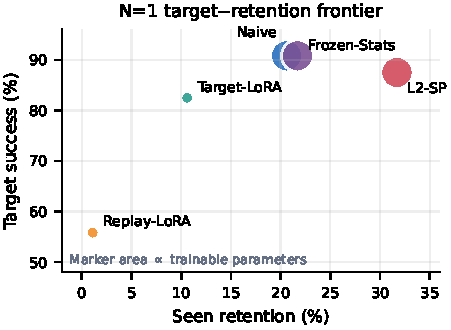
\includegraphics[width=0.50\textwidth]{method_frontier.pdf}
\end{center}

\clearpage

\section{\texorpdfstring{\(N=1\)}{N=1} per-task and per-seed results}

Target is out of 20 rollouts. Retention is out of 30 rollouts
(three frozen probes, ten seeds each).

\begin{longtable}{@{}lllrrrr@{}}
\toprule
Method & Target task & Seed & Target & Retention & Train wall & Peak VRAM\\
\midrule
\endfirsthead
\toprule
Method & Target task & Seed & Target & Retention & Train wall & Peak VRAM\\
\midrule
\endhead
Naive & Drawer & 42 & 17/20 & 4/30 & 199.1 s & 7,540 MiB\\
Naive & Drawer & 123 & 19/20 & 2/30 & 199.4 s & 7,540 MiB\\
Naive & Bowl & 42 & 20/20 & 10/30 & 162.2 s & 7,540 MiB\\
Naive & Bowl & 123 & 20/20 & 10/30 & 162.0 s & 7,540 MiB\\
Naive & Wine & 42 & 16/20 & 6/30 & 127.2 s & 7,540 MiB\\
Naive & Wine & 123 & 17/20 & 5/30 & 126.9 s & 7,540 MiB\\
\midrule
Target-LoRA & Drawer & 42 & 15/20 & 0/30 & 314.7 s & 6,944 MiB\\
Target-LoRA & Drawer & 123 & 8/20 & 1/30 & 315.0 s & 6,938 MiB\\
Target-LoRA & Bowl & 42 & 20/20 & 9/30 & 229.7 s & 6,944 MiB\\
Target-LoRA & Bowl & 123 & 20/20 & 7/30 & 229.3 s & 6,944 MiB\\
Target-LoRA & Wine & 42 & 19/20 & 1/30 & 187.0 s & 6,882 MiB\\
Target-LoRA & Wine & 123 & 17/20 & 1/30 & 188.2 s & 6,944 MiB\\
\midrule
Replay-LoRA & Drawer & 42 & 3/20 & 0/30 & 435.9 s & 6,944 MiB\\
Replay-LoRA & Drawer & 123 & 3/20 & 0/30 & 436.0 s & 6,944 MiB\\
Replay-LoRA & Bowl & 42 & 20/20 & 1/30 & 332.3 s & 6,944 MiB\\
Replay-LoRA & Bowl & 123 & 20/20 & 1/30 & 332.3 s & 6,944 MiB\\
Replay-LoRA & Wine & 42 & 8/20 & 0/30 & 159.7 s & 6,944 MiB\\
Replay-LoRA & Wine & 123 & 13/20 & 0/30 & 159.9 s & 6,944 MiB\\
\bottomrule
\end{longtable}

\subsection{Probe totals and instability}

\begin{center}
\begin{tabular}{@{}lrrr@{}}
\toprule
Method & Black bowl / plate & Drawer / bowl & Book / caddy\\
\midrule
Naive & 21/60 & 14/60 & 2/60\\
Target-LoRA & 12/60 & 7/60 & 0/60\\
Replay-LoRA & 2/60 & 0/60 & 0/60\\
\bottomrule
\end{tabular}
\end{center}

Target-LoRA is stable for Bowl (20/20 for both seeds) but not for Drawer
(15/20 vs.\ 8/20). The result supports adding more train seeds before a final
method claim. The three probes should also be expanded only after the method is
locked, so probe selection cannot become another form of tuning.

\section{Training diagnostics}

\subsection{Seen expert}

The full 100k run takes 38,870 seconds (10 h 47 min 50 s), processes 3.2M
samples, reserves 7,536 MiB at the final logged step, and ends at loss 0.23494.

\begin{center}
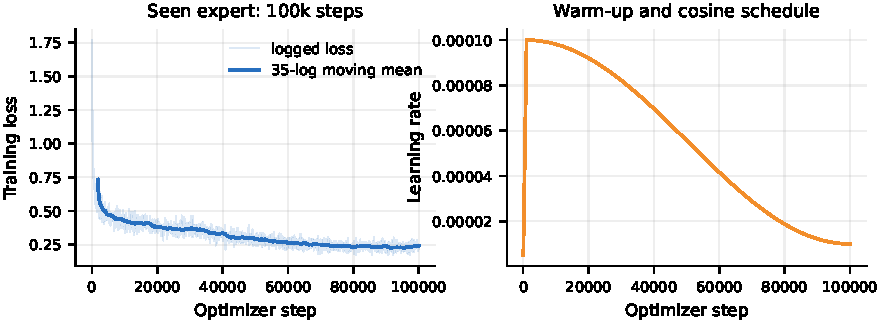
\includegraphics[width=\textwidth]{seen_training.pdf}\\[-2pt]
{\small\textbf{Figure A1.} Seen training loss and frozen optimizer schedule.}
\end{center}

\clearpage

\subsection{Naive target training}

The target stop is 100 dataset epochs capped at 12k optimizer steps.
Because datasets are small, actual step counts depend on task length and \(N\).
For \(N=1\), final logged steps are 300--500. Curves below show the median and
interquartile range over three tasks and two train seeds at each budget.

\begin{center}
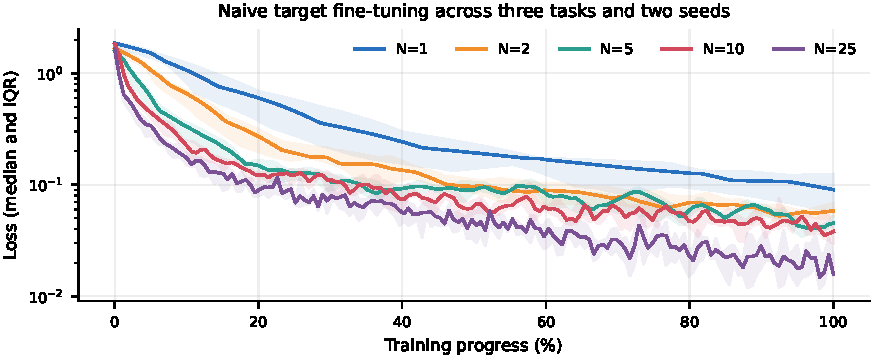
\includegraphics[width=\textwidth]{baseline_training.pdf}\\[-2pt]
{\small\textbf{Figure A2.} Naive fine-tuning losses. Training progress is normalized because run lengths differ.}
\end{center}

\subsection{LoRA and replay diagnostics}

\begin{center}
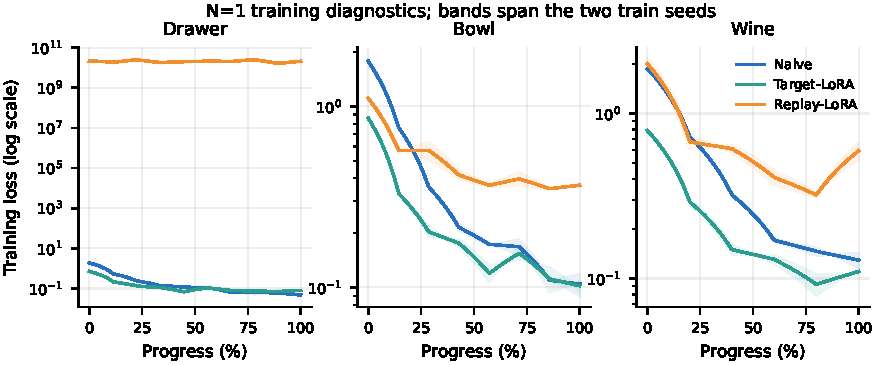
\includegraphics[width=\textwidth]{lora_diagnostics.pdf}\\[-2pt]
{\small\textbf{Figure A3.} \(N=1\) loss by task and method; bands span seeds 42 and 123.}
\end{center}

Replay-LoRA Drawer is numerically pathological. The first Drawer demonstration
has gripper standard deviation \(10^{-6}\), while seen replay contains both
gripper states. The target-only normalizer therefore creates extreme
standardized replay targets. Final Drawer losses are \(1.44\times10^{10}\) and
\(2.72\times10^{10}\). Bowl and Wine do not show the same explosion, so this
does not explain their full retention loss. A follow-up should log loss and
gradient norms by source and by action dimension before any update.

\subsection{Compute and concurrency}

\begin{center}
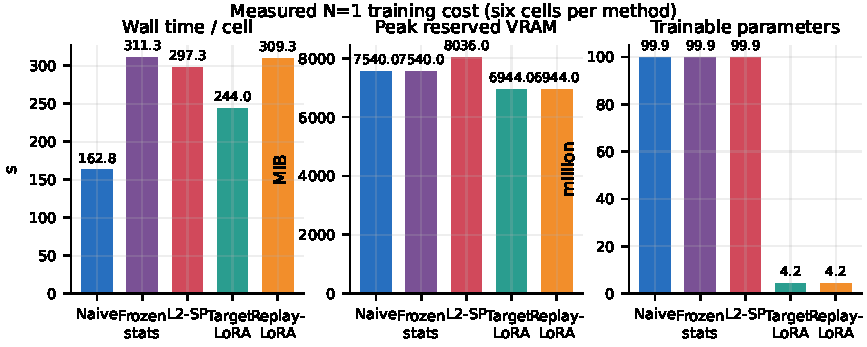
\includegraphics[width=\textwidth]{compute_cost.pdf}\\[-2pt]
{\small\textbf{Figure A4.} Mean wall time, per-process peak reserved VRAM, and trainable parameter count.}
\end{center}

A bounded concurrency benchmark compared two and four simultaneous jobs.
Four jobs improved aggregate throughput by about 1.6 times and reserved about
27,776 MiB in total on a 97 GB RTX PRO 6000. The official 12-cell LoRA grid
finished in 1,007.7 seconds (16 min 48 s) from first start to last finish.
Wall time per cell includes this concurrent load and is not an isolated
microbenchmark.

\clearpage

\section{Controls, integrity, and artifact map}

\subsection{Language control}

All 60 correct/wrong pairs use identical initial-state fingerprints.
The frozen policy changes its trajectory when the instruction changes,
but success is too low to prove strong language grounding.

\begin{center}
\begin{tabular}{@{}lrrrr@{}}
\toprule
Task & Correct & Wrong & Mean action \(L_2\) & Mean cosine gap\\
\midrule
Drawer & 1/20 & 0/20 & 0.5820 & 0.3273\\
Bowl & 0/20 & 0/20 & 0.9982 & 0.7731\\
Wine & 0/20 & 0/20 & 0.9661 & 0.6626\\
\bottomrule
\end{tabular}
\end{center}

\subsection{Normalization 2-by-2 control}

\begin{center}
\begin{tabular}{@{}llrr@{}}
\toprule
Weights & Statistics & Success & Interpretation\\
\midrule
Frozen seen & \code{libero_90} & 12/15 & expected seen competence\\
Frozen seen & target overlay & 0/60 & statistics alone break deployment\\
Adapted target & target overlay & 0/60 & confounded earlier retention\\
Adapted target & \code{libero_90} & 6/60 & corrected weight test\\
\bottomrule
\end{tabular}
\end{center}

The old 0/900 overlay result is retained as a deployment-normalization warning,
not reported as catastrophic forgetting. The corrected retention grid checks
checkpoint SHA, statistics digest, task/train/eval seeds, and frozen initial
state fingerprints.

\subsection{Task 2 integrity}

All 12 LoRA training cells are complete and have unique final weight hashes.
All 240 target records and 360 retention records passed exact checks for:

\begin{itemize}
  \item frozen base SHA and method identity;
  \item task, train seed, evaluation seed, and first-demo episode;
  \item target or seen statistics suite and digest;
  \item fixed initial-state fingerprint;
  \item replay source restricted to \code{libero_90}, with no selection based on probes.
\end{itemize}

The code state for the Task 2 grid is clean commit
\sha{cebe04d9ab408eaa37c7ab0249d48fe915ae7b36}.
The repository test suite reports 304 passed and 8 skipped.

\subsection{Artifact map}

\begin{tabularx}{\textwidth}{@{}lX@{}}
\toprule
Evidence & Location\\
\midrule
Main paper source & \artifact{report/latex/paper.tex}\\
Frozen predictions & \artifact{predictions.md}\\
Seen training log & \artifact{/mnt/vla/runs/seen__expert__libero90__nall__s42__20260822T010019Z__gd4b8fb8/metrics.csv}\\
Zero-shot export & \artifact{/mnt/vla/eval/zero_shot_v2_seen_stats/report/summary.md}\\
Language control & \artifact{/mnt/vla/eval/language_control/report/summary.md}\\
Naive \(N=1,2\) results & \artifact{/mnt/vla/validation/TODO28_n12/results.md}\\
Corrected retention & \artifact{/mnt/vla/validation/TODO28_retention_libero90/retention.md}\\
Task 2 result & \artifact{report/tables/task2_n1_results.md}\\
Task 2 training & \artifact{/mnt/vla/runs/task2_n1}\\
Task 2 target eval & \artifact{/mnt/vla/eval/task2_n1/target}\\
Task 2 retention & \artifact{/mnt/vla/eval/task2_n1/retention_libero90}\\
\bottomrule
\end{tabularx}

\subsection{Recommended next experiment}

Before training, audit one mixed replay batch in the shared action coordinate
system and report source counts, per-source/per-dimension normalized ranges,
losses, and gradient norms. Then preregister one normalization-safe replay
variant or a frozen-policy distillation penalty. Lock the method before
evaluating a broader seen-task set, and report the complete target--retention
Pareto frontier rather than choosing one checkpoint by target success.

\end{document}
